% The first command in your LaTeX source must be the \documentclass command.

\documentclass[sigconf]{acmart}
 % Do not change for ITiCSE'20

\settopmatter{printacmref=true}
  % mandatory for ITiCSE'20

\fancyhead{}
  % do not delete this code.

\usepackage{balance}
  % for creating a balanced last page (usually last page with references)

% defining the \BibTeX command - from Oren Patashnik's original BibTeX documentation.
\def\BibTeX{{\rm B\kern-.05em{\sc i\kern-.025em b}\kern-.08emT\kern-.1667em\lower.7ex\hbox{E}\kern-.125emX}}
    
% Rights management information. 
% This information is sent to you when you complete the rights form.
% These commands have SAMPLE values in them; it is your responsibility as an author to replace
% the commands and values with those provided to you when you complete the rights form.
%
% These commands are for a PROCEEDINGS abstract or paper.
\copyrightyear{2020}
\acmYear{2020}
\setcopyright{acmcopyright}
\acmConference[ITiCSE '20]{Proceedings of the 2020 ACM Conference on Innovation and Technology in Computer Science Education}{June 15--19, 2020}{Trondheim, Norway}
\acmBooktitle{Proceedings of the 2020 ACM Conference on Innovation and Technology in Computer Science Education (ITiCSE '20), June 15--19, 2020, Trondheim, Norway}
\acmPrice{15.00}
\acmDOI{10.1145/3341525.3387372}
\acmISBN{978-1-4503-6874-2/20/06}


% Submission ID. 
% Use this when submitting an article to a sponsored event. You'll receive a unique submission ID from the organizers
% of the event, and this ID should be used as the parameter to this command.
%\acmSubmissionID{123-A56-BU3}


% end of the preamble, start of the body of the document source.

\begin{document}

\fancyhead{}
  % do not delete this code.


% The "title" command has an optional parameter, allowing the author to define a "short title" to be used in page headers.
\title{Resilience and Effective Learning in First Year Undergraduate Computer Science}


% The "author" command and its associated commands are used to define the authors and their affiliations.
% Of note is the shared affiliation of the first two authors, and the "authornote" and "authornotemark" commands
% used to denote shared contribution to the research.

\author{Tom Prickett, Julie Walters, Longzhi Yang}
\affiliation{%
 \institution{ Northumbria University}
 \city{Newcastle upon Tyne}
 \country{UK}
 }
\email{tom.prickett@northumbria.ac.uk, Julie.Walters@northumbria.ac.uk, Longzhi.Yang@northumbria.ac.uk}

\author{Morgan Harvey}
\affiliation{
 % \department{Department}
  \institution{University of Sheffield}
  \city{Sheffield} 
  \country{UK}
}
\email{m.harvey@sheffield.ac.uk}

\author{Tom Crick}
\orcid{0000-0001-5196-9389}
\affiliation{%
\institution{Swansea University}
\city{Swansea}
\country{UK}
 }
\email{thomas.crick@swansea.ac.uk}


%
% By default, the full list of authors will be used in the page headers. Often, this list is too long, and will overlap
% other information printed in the page headers. This command allows the author to define a more concise list
% of authors' names for this purpose.
\renewcommand{\shortauthors}{Prickett, et al.}

%
% The abstract is a short summary of the work to be presented in the article.
\begin{abstract}
Many factors have been shown to be important for supporting effective learning and teaching -- and thus progression and success -- in higher education. While factors such as key introductory-level (CS1) knowledge and skills, as well as pre-university learning and qualifications, have been extensively explored, the impact of measures of positive psychology are less well understood for the discipline of computer science. University study can be a period of significant transition for many students; therefore an individual's positive psychology may have considerable impact upon their response to these challenges. This work investigates the relationships between effective learning and success (first year performance and attendance) and two measures of positive psychology: Grit and the Nicolson McBride Resilience Quotient (NMRQ).

Data was captured by integrating Grit (n=58) and Resilience (n=50) questionnaires and related coaching into the first year of the undergraduate computer science programme at a single UK university. Analyses demonstrate that NMRQ is significantly linked to attendance and performance for individual subjects and year average marks; however, this was not the case for Grit. This suggests that development of targeted interventions to support students in further developing their resilience could support their learning, as well as progression and retention. Resilience could be used, in concert with other factors such as learning analytics, to augment a range of existing models to predict future student success, allowing targeted academic and pastoral support.
\end{abstract}

%
% The code below is generated by the tool at http://dl.acm.org/ccs.cfm.
% Please copy and paste the code instead of the example below.
%
\begin{CCSXML}
<ccs2012>
<concept>
<concept_id>10003456.10003457.10003527</concept_id>
<concept_desc>Social and professional topics~Computing education</concept_desc>
<concept_significance>500</concept_significance>
</concept>
</ccs2012>
\end{CCSXML}

\ccsdesc[500]{Social and professional topics~Computing education}
%%
%% Keywords. The author(s) should pick words that accurately describe
%% the work being presented. Separate the keywords with commas.
\keywords{
  Resilience,
  Effective Learning,
  %Engagement,
  Progression,
  Success,
  Learning Analytics
}



%
% This command processes the author and affiliation and title information and builds
% the first part of the formatted document.
\maketitle

\section{Introduction}
It has long been recognised that competence and resilience are important in maintaining effective learning and achieving successful outcomes in higher education~\cite{Marsten95,Walker2006,Holdsworth2018}. Competence can be seen as current performance; so for first year students it will initially be determined by the knowledge, skills and experiences students arrive with and further develop as part of their studies. In the context of computer science (CS), there are specific disciplinary challenges; for example, learning programming for the first time remains a significant hurdle~\cite{davenport-et-al:latice2016,murphy-et-al:programming2017,simon-et-al:sigcse2018}, with a range of issues impacting failure rates~\cite{Porter:2013:HFR:2445196.2445250,Watson:2014:FRI:2591708.2591749}. Competence, however, is not all -- \textit{positive psychology ~\cite{Seligman90}} - a reflection of optimism in the face of challenges is also important in maintaining effective learning and can be enhanced through educational interventions \cite{Walker2006,Holdsworth2018}.

% \begin{comment}
% Student retention and progression is a key issue in higher education as every student accepted represents a significant commitment in time, resources and effort, and considerable pressure has been placed on universities to improve retention and progression rates for a number of years~\cite{Crosling2008}. Rates vary considerably by discipline and research has shown that Computer Science suffers from particularly poor retention~\cite{Gordon}. Learning programming for the first time remains a challenge~\cite{Watson:2014:FRI:2591708.2591749} with the failure rate on follow-on modules also reported as being high~\cite{Porter:2013:HFR:2445196.2445250}. As such there is continuing interest in understanding the factors that contribute to these poor results and student success.
% \end{comment}

% \begin{comment}
% An individual's positive psychology~\cite{Seligman90} is a reflection of their optimism in the face of challenges. First year university study can be a period of significant transition for all students~\cite{Tinto1975} and, as such, an individual's positive psychology may have an impact upon their response to challenges of transition to higher education. This paper focuses upon the analysis of  the relationships between positive psychology measures and first year student success and attendance at a UK university. In the UK, computer science benefits from being a discipline accessible to those who have not studied computing before. As such most degrees assume little prior knowledge and teach \textit{ab initio}. This may contribute to the challenges of transition faced by some first year computer science students, potentially making positive psychology of even greater relevance.
% \end{comment}

Student engagement and success are key issues in higher education -- attending university demands a sizeable commitment on the part of an individual student (intellectually of course, but also financially, as well as ``socially''), and every student accepted represents a significant commitment in time, resources and effort on behalf of a university. Student engagement ``has come to refer to how involved or interested students appear to be in their learning and how connected they are to their classes, their institutions, and each other''~\citep[p.~38]{Axelson2010} and, among other factors, can be measured based on time on task~\cite{kuh2009national} and educational outcomes.

University study can be a period of significant transition for all students~\cite{Tinto1975} and, as such, an individual's psychology may have an impact upon their response to challenges of transition to higher education. This work considers two key aspects of positive psychology: grit and resilience, which are similar but subtly different. Grit is defined as the passion and perseverance for a singularly important goal~\cite{Duckworth2007}; while resilience is how well an individual can adapt to challenges. In the context of this work, resilience is defined as a quality that helps you turn adversity into advantage and threat into opportunity~\cite{Clarke2010}.  

% \begin{comment}
% There are number of measures for effective learning that could be included. Should it be the results a student obtains? Should it be a measure related to the students perception of the quality (possibly via a student perception survey)? This would be challenging to obtain in an un-biased manner if the link to the original student and other factors is to be maintained. Should it be the extent to which it enables students to achieve their own aspirations and goals (maybe employment or further study related)? This would be difficult to obtain for first year students in a timely manner. 

% One readily available measure related to 'time and effort' is attendance. One measure of the outcome of 'educationally purposeful activities' is student results. As such a students results was selected as a proxy measure for student engagement and  effective learning.
% \end{comment}

The CS education research community has been working on predicting student success for a number of years~\cite{Robins2010}. A number of sociological, psychological and economical models have been proposed in the literature for retention prediction, with some success~\cite{Seidman2012}. Recently, artificial intelligence and machine learning approaches -- especially in the context of a wider higher education push on learning analytics~\cite{jiscla:2020} -- have been widely applied in retention prediction. Existing work considers socio-demographic variables (e.g. age, gender, ethnicity, education, work status, and disability) and study environment variables, such as course programme and course block (e.g.~\cite{Liao:2019:EVD:3287324.3287407}). However, there is limited published work related to the prediction of a computer science student's overall results and attendance based on measures of positive psychology. As such, in the context of a UK University this work seeks to:
\begin{enumerate}
    \item RQ1: explore and evaluate the relationship between first year CS student success and attendance using Duckworth's 12-item Grit scale;
    \item RQ2: explore and evaluate the relationship between first year CS student success and attendance using Nicholson McBride Resilience Quotient (NMRQ).
\end{enumerate}
In this research we are not developing a model for predictive purposes, but are instead employing the techniques to assess the strength of relationship between different factors.

\section {Background}

% \begin{comment}
% Student retention and success are critical issues for education, based on generally three broad rationales~\cite{Wood2014}. Due to this, intensive work has been carried out in this area from a wide range of aspects. In addition, actions have been taken by governments to improve retention rates, such as the ``American Graduation Initiative'' \cite{Wood2014} and the UK Teaching Excellence Framework (TEF)~\cite{Gunn2018}.
% \end{comment}

Learning means different things to different learners \cite{saljo1979learning, Ramsden1992}. Effective learning is when this learning achieves the desired result \cite{kolb2014}. There is a considerable corpus of work related to the promotion of effective learning, which is significantly impacted by learner engagement, and blockers to it~\cite{kolb2014, Ramsden1992}. Early work related to the blockers of learning focusing on student retention was carried out by Tinto~\cite{Tinto1975}, who produced a model of student attrition, which suggested that student retention is influenced by student attributes and experience combined with institutional factors. These attributes include: previous educational input, family history and the individual's own abilities whereas the institutional factors focus on achievement while at university and faculty interactions. Since then much work has focused on student retention~\cite{Barbera2017,Chen2012}, largely by exploring individual elements of this model and focusing primarily on institutional factors. A number of studies have also investigated the relationships between student success and student attributes, including gender~\cite{Lishinski:2016:LPG:2960310.2960329}, pre-entry grades~\cite{Peterson1979} and previous experience~\cite{Ramalingam:2004:SMM:1026487.1008042}. An alternative, and more positive, approach has been to consider the challenges in the curricula studied; so-called ``threshold concepts'' and ``troublesome knowledge''~\cite{Land2012}. In the domain of CS, threshold concepts have be argued to be largely related to programming~\cite{Sanders:2016:TCC:2999541.2999546}, leading to research related to success seen through the lens of programming (commonly fundamental programming or ``CS1''). This has been productive but can been argued to leave a gap in our understanding of factors that can be predictors of success~\cite{Liao:2019:EVD:3287324.3287407,Liao:2016:LEI:2960310.2960315,Castro-Wunsch:2017:ENN:3017680.3017792,Quille:2018:PPS:3197091.3197101}. In particular, in the case of ``troublesome knowledge'', learners may need to perform in the face of adversity. Hence a learners' positive psychology and the further enhancement to that positive psychology may be beneficial to learning such ``troublesome knowledge''.

Seligman argued that there is {\em'third factor -optimism or pessimism- that matters as much as talent or desire'}\cite[p.~13]{Seligman90}. Seligman goes further and argues that you can learn to be both optimistic or helpless, thereby providing the foundations for {\em positive psychology}. To have achieved access to university study, learners must have acquired learning capabilities, disciplinary capabilities and some learning or academic resilience. As part of university study, learners will enhance disciplinary capabilities, learning capabilities and learning resilience.  Many socioeconomic and societal issues as well as context may influence a learners beliefs about their academic capabilities is related to their motivation to achieve and ability to persevere through difficult challenges~\cite{ZIMMERMAN200082,Bandura1977} and hence their resilience. 
 
Duckworth et al. building on the work of Seligman, defined the term grit as ``perseverance and passion for long term goals''~\cite{Duckworth2007}, reflecting the desire to achieve and determination to overcome challenges, which may be as important as raw talent. Duckworths' work successfully correlates grit with higher education success, however, it does not claim to precisely predict, instead explaining a significant amount of variation in success. Grit is not without criticism; the extent to which it it is correlated with the factors it is purported to predict may vary in different countries~\cite{Datu2016, Tyumeneva2017}, suggesting there may be cultural differences that have an influence upon its effectiveness. 

A large number of scales have been developed in order to measure resilience; in this work we have chosen to use the NMRQ~\cite{Clarke2010}. NMRQ is a shortened version of the Nicholson McBride Resilience Questionnaire (12 questions rather then 64) \cite{Clarke2010}. NMRQ measures {\em'the ability bounce back from tough times or even triumph in the face of adversity; to display tenacity, but not at the expense of reason'\cite{Clarke2010}} NMRQ has been deployed successfully in a number of contexts, including professional development of doctors~\cite{Tregoningg251} and retention of underrepresented populations at university~\cite{Daniels2015} and in several commercial contexts~\cite{Clarke2010}. This definition of resilience is consistent with the educational challenges of higher education study, it is a wider in scope than Grit including a variety of aspects of positive psychology.

Recent work has mapped provision, pedagogy and practice to deliver introductory programming (``CS1'') as part of undergraduate computer science (and cognate) degree programmes in UK universities~\cite{davenport-et-al:latice2016,murphy-et-al:programming2017,simon-et-al:sigcse2018}. Prediction of introductory programming performance based upon machine learning and source code snapshots has had some success~\cite{Ahadi:2015:EML:2787622.2787717,Castro-Wunsch:2017:ENN:3017680.3017792}, as has prediction based upon in-class clicker questions ~\cite{Liao:2016:LEI:2960310.2960315,Liao:2019:RML:3308443.3277569}. The Predict Student Success (PreSS) model, a composite model based upon programming self-efficacy, mathematical ability based on a high school mathematics exit examination and number of hours per week a student plays computer games achieved a 77.5\% success rate in predicting CS1~\cite{Quille:2018:PPS:3197091.3197101}. The prediction of CS1 performance based upon Grit~\cite{Sigurdson:2018:EGC:3279720.3279743} has been attempted; however, there is limited published work related to the inclusion of positive psychology (including grit and resilience) and attendance within these models for the prediction of success with CS1 and wider success.

\section {Method}
This paper reports the results of a study conducted in the Department of Computer and Information Sciences at a mid-range UK university, which offers a number of undergraduate and postgraduate programmes in computer science, information science, networking and cyber security and digital forensics. The department currently has 67 full-time members of academic staff and approximately 1,200 students enrolled across all the programmes.

%\subsection {Data sets}

\begin{table*}[ht]
\caption{Information about Subjects (Modules) constituting first year of the Computer Science programme.}
\begin{tabular}{llll}
\hline
\textbf{ID} & \textbf{Subject / Module} & \textbf{Median mark} & \textbf{Topics} \\
\hline
CS1  & Programming (Java)         & 63.25        & Variables, methods, Objects, conditionals, loops, arrays          \\
DB  & Relational Databases       & 61        & Database fundamentals, SQL, ERDs, information security          \\
Web  & Web Technologies         & 69.5      & Mark-up languages, HTML, CSS, usability, client-side processing, web security          \\
CSFund  & Computing Fundamentals & 80        & Logic, von Neumann architectures, binary representation, maths foundations          \\
SysA  & Systems Analysis        & 71        & Data collection techniques, UML Modelling, professional issues                 
\end{tabular}
\label{tab:module_info}
\end{table*}

{\em Data sets.}
Data was obtained by integrating two surveys, grit and resilience, into the delivery of a first year core subject (Systems Analysis/SysA) on a Computer Science degree during the second week of teaching in the second semester (in early February) in a class delivered by a member of the research team. Students were asked to complete the surveys using the University's Electronic Learning Platform and afterwards were encouraged to reflect upon their results. The students were supported in the interpretation of their results and guidance was provided regarding strategies they could adopt to improve them in the context of their degree studies. The study was approved by the University's ethics board and students were specifically asked for consent to use their data for research. Data on student performance was obtained at the end of the teaching year and consists of the results from five different subjects over both semesters of the academic year as well as attendance data over the year. Table~\ref{tab:module_info} provides information about the five subjects and the average (median) mark obtained by students in the data set for each.

The data set is comprised of the students who formally consented to use their survey, giving a sample of 50 who completed the resilience survey and 58 who competed the grit survey. Both surveys comprised 12 items, phrased as statements, answered on five-point Likert scales from ``{\emph{strongly disagree (1)}}'' to ``{\emph{strongly agree (5)}}''. Scores for the resilience survey are added together, yielding total scores between 12 and 60, while those for the grit scale are averaged to produce mean values.

To explore the significance of the relationships, the problem was framed as one of prediction. Therefore, is necessary to separate the students into classes and, as we are primarily interested in performance, we split the students by means of their marks. The sample was, broadly speaking, high performing students and, as such, we used the median overall mark across all subjects (70) to produce two classes. This is also appropriate as it happens to be the cutoff for a 1st class honours degree in the UK (the highest honours degree you can achieve). It has been widely reported in the UK media that there has been an increase in the number of students struggling to cope and seeking counselling. Rising costs of study and fear of failure to succeed (including achieving a `good degree') appear to be factors~\cite{BBC}; as such to many students this is becoming the grade boundary that is seen as a success.

%\subsection{Model generation and analysis}
{\em Model generation and analysis.}
We used logistic regression to perform classification between the high-performing and low-performing binary student classes. We employed logistic regression as it works well with a small number of input features and benefits from being relatively simple to use and explain. The model outputs a number in the range $[0,1]$, which represents the probability that the candidate data point belongs to the positive class (i.e. a high-performing student). Analysis was conducted using the R statistical programming environment and, more specifically, the Generalised Linear Model (glm) library, which also permits automatic feature selection by means of Akaike information criterion-based (AIC-based) stepwise regression.

Before producing any regression models, we used correlation analysis to understand whether the resilience and grit scale results correlate with student performance, both on average over the year and for individual subjects, and attendance. Correlation coefficients were tested for significance using t-tests with the null hypothesis that the coefficient is not significantly different from 0. 

The quality of the regression models was assessed by their ability to accurately predict the performance or attendance class. This is assessed by evaluating the Area Under the Curve (AUC) of the Receiver Operating Characteristic (ROC) curve and classifier accuracy. For both measures, a value closer to 1.0 implies a better model and, therefore, better predictive performance. 

\section {Results}
Correlation analysis was first used to provide an indication as to whether or not grit and resilience are predictive of student performance and attendance. If there is a high degree of correlation between a psychological measure and a measure of performance or level of attendance then it is likely that the former will be predictive of the latter. This was followed by the use of logistic regression models to analyse this predictive performance.

%\subsection{Correlation analysis}

\begin{figure}[h]
\centering
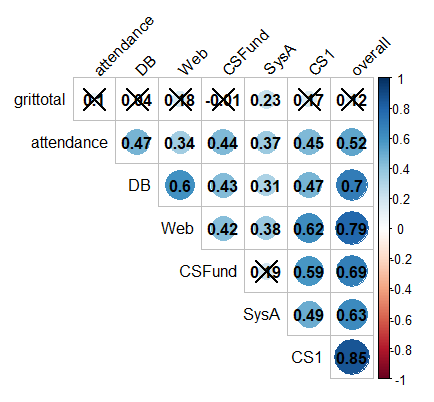
\includegraphics[width=.9\linewidth]{images/cor_plot_grit.png}
\caption{Correlation matrix of grit score against performance and attendance.}
\label{fig:cor_grit} 
\end{figure}

\begin{figure}[h]
\centering
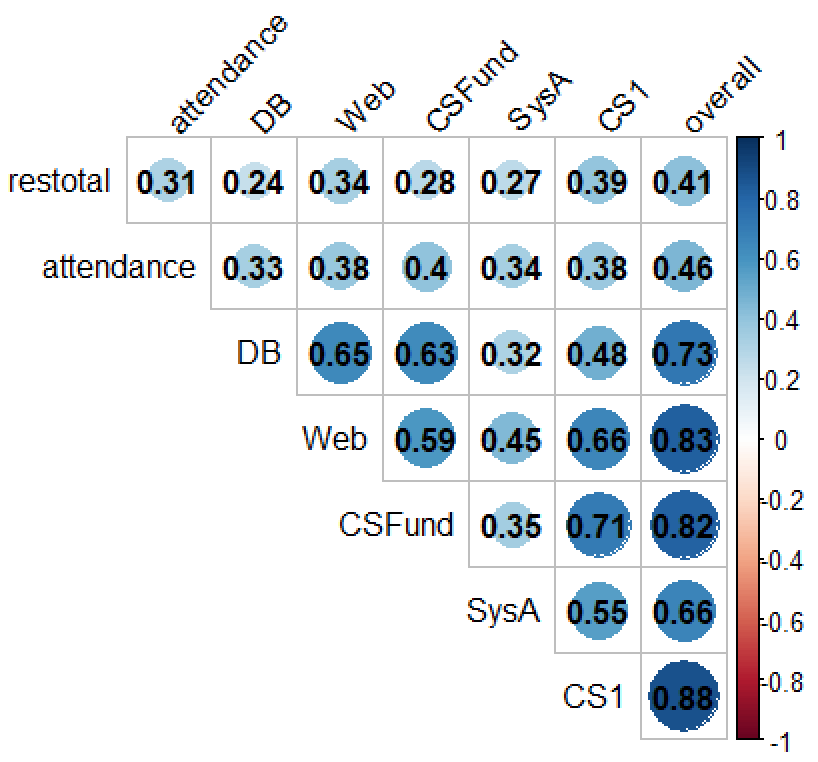
\includegraphics[width=.9\linewidth]{images/cor_plot_res.png}
\caption{Correlation matrix of resilience score against performance and attendance.}
\label{fig:cor_res} 
\end{figure}

{\em Correlation analysis.}
Figures~\ref{fig:cor_grit} and \ref{fig:cor_res} show matrices of the results of the correlation analysis. The size and depth of colour of the circles indicates the degree of the correlation, with blue indicating a positive correlation and red indicating a negative one. Any cells of the matrix filled with a cross ($X$) indicates that the correlation coefficient is not significantly different from 0 and, therefore, that the relationship between the two features is not significant.

These results indicate that, with the exception of the {\em SysA} subject, the total grit score (Figure~\ref{fig:cor_grit}) does not significantly correlate with student performance or attendance. However, in the case of resilience (Figure~\ref{fig:cor_res}), we see that this psychological measure correlates significantly with student performance for all subjects, as well as their average performance over the year, and with attendance. It is also worth noting that attendance correlates significantly with performance over all subjects, encouragingly suggesting that actually turning up to classes really does have a benefit! It is also notable that, barring a single exception, the performance for all subjects and overall performance are all significantly correlated with each other - if a student performs well on one subject then they tend to perform well generally. 

%\subsection{Predicting performance with Duckworth's 12-item Grit scale}

\begin{table}[]
\caption{Prediction performance of various models. $\cdot$ $p < 0.1$; * $p < 0.05$}
\begin{tabular}{lllll}
\hline
\multicolumn{1}{|l|}{\textbf{Model}} & \multicolumn{1}{l|}{\textbf{$x_1$}} & \multicolumn{1}{l|}{\textbf{p value}} & \multicolumn{1}{l|}{\textbf{Accuracy}} & \multicolumn{1}{l|}{\textbf{AUC}} \\ \hline
overall $\sim$grit                   & 0.385                              & 0.385                                 & 0.59                                   & 0.555                             \\
SysA $\sim$grit                      & 0.724                              & 0.119                                 & 0.64                                   & 0.636  \\ \hline
overall $\sim$resilience             & 0.135                              & 0.042 *                               & 0.66                                   & 0.671                             \\
CS1 $\sim$resilience                 & 0.154                              & 0.026 *                               & 0.68                                   & 0.691                             \\
DB $\sim$resilience                  & 0.151                              & 0.027 *                               & 0.64                                   & 0.681                             \\
Web $\sim$resilience                 & 0.106                              & 0.106                                 & 0.59                                   & 0.616                             \\
CSFund $\sim$resilience              & 0.181                              & 0.015 *                               & 0.7                                    & 0.713                             \\
SysA $\sim$resilience                & 0.08                               & 0.192                                 & 0.6                                    & 0.637                             \\
attendance$\sim$resilience           & 0.125                              & 0.058 $\cdot$                               & 0.56                                   & 0.657                             \\ \hline
overall $\sim$best\_model            & NA                                 & NA                                    & 0.76                                   & 0.830                            
\end{tabular}
\label{tab:model_performance}
\end{table}

\begin{figure} [h]
\centering
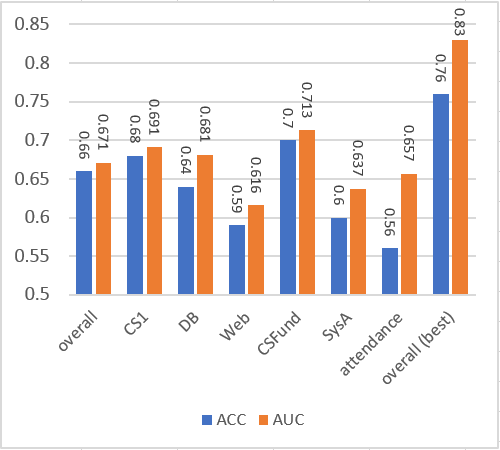
\includegraphics[width=.9\linewidth]{images/model_performance.png}
\caption{Performance of resilience-based models in terms of accuracy (ACC) and ROC AUC.}
\label{fig:model_performance} 
\end{figure}

{\em Predicting performance with Duckworth's 12-item Grit scale.}
The first two rows of Table~\ref{tab:model_performance} summarise the performance of the overall grit score as a predictor of overall student performance and student performance in the {\em SysA} subject. Although the accuracy and AUC values do suggest that grit may have some relationship with student performance, it is extremely weak and is not significant in either case. We do not show results for the other subjects and attendance as these are weaker still. These results suggest that Duckworth's 12-item grit scale does not have a strong relationship with undergraduate computer science student performance or attendance. 

%\subsection{Predicting performance with Nicholson McBride Resilience Quotient}
\begin{figure} [h]
\centering
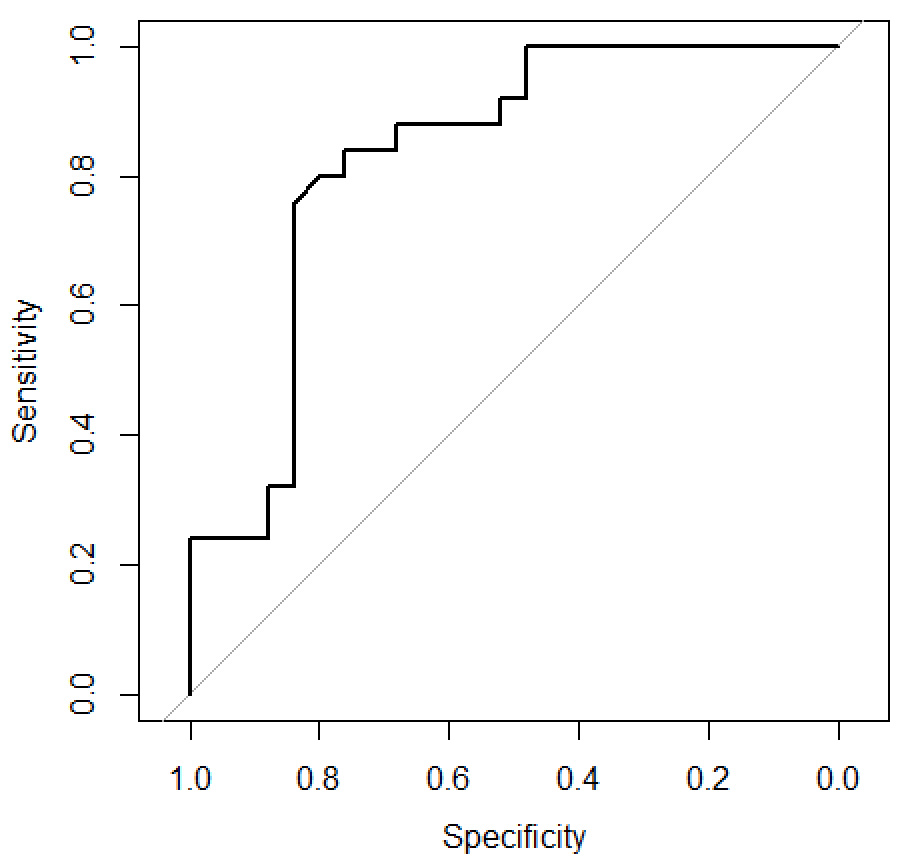
\includegraphics[width=.9\linewidth]{images/ROC_best_model.png}
\caption{ROC curve plot of best-performing resilience composite model (``{\em best}'').}
\label{fig:roc_curve} 
\end{figure}

{\em Predicting performance with NMRQ}
The remaining 8 rows of Table~\ref{tab:model_performance} summarise the performance of models built using the NMRQ (resilience) results as predictors of student performance and attendance. To aid comparison, these results are visualised in Figure~\ref{fig:model_performance}. Overall resilience score (the middle seven rows) is a significant predictor of overall student performance as well as performance on the individual subjects {\em CS1}, {\em DB} and {\em CSFund}, although this is not the case for the subjects {\em Web}, {\em SysA} or for overall attendance. Predictive accuracy and AUC are particularly high for {\em CS1}, the introduction to programming subject (accuracy = 0.68, AUC = 0.691), and for {\em CSFund}, which introduces students to core fundamental computer science concepts and ideas (accuracy = 0.7, AUC = 0.713).

The final row of Table~\ref{tab:model_performance} and final two bars of Figure~\ref{fig:model_performance} summarise the performance of a different model, which we refer to as ``{\em best}''. This model uses the individual component items of the NMRQ as predictor variables, rather than the single variable (their sum) used previously. Not all of these individual items will be predictive of performance and, as should be the case for any well-designed scale, some of the items strongly correlate with each other. As such, we used  automatic feature selection by means of AIC-based stepwise regression to obtain a quasi-optimal model. This {\em best} model comprises six items from the 12-item NMRQ scale (question \# 2, 5, 6, 9, 10 and 11). This model was obtained after seven steps of reducing the original 12-item model. The results demonstrate that this model has considerably better predictive power than the sum of the individual scores on its own. In predicting student performance over the whole year, it achieves an accuracy on our data of 0.76 and a AUC of 0.83, with compares favourably with the performance of the model with the single predictor, which achieved an accuracy of 0.66 and an AUC of 0.671. Figure~\ref{fig:roc_curve} visualises the ROC curve of this model, demonstrating that both specificity and sensitivity of the model are high for a large range of threshold values.

\section{Discussion}
%\subsection{Discussion related to correlation analysis}
{\em Discussion related to correlation analysis}
%\subsubsection{Grit scores and performance}
Grit scores were found to not be significantly correlated with the overall average of the first year or with most of the first year subjects, including CS1. This is consistent with other similar research~\cite{Sigurdson:2018:EGC:3279720.3279743} and serves to support the findings that, for some reason (possibly cultural factors), grit score is not related with performance on CS1 or to overall first year computer science performance in the UK. The only exception to this was for the Systems Analysis/SysA subject, whose outcomes were significantly correlated with grit scores. This may be explained by the mode of assessment for this subject. As part of this assessment students are required identify a potential system development and then to engage in a data collection exercise involving live data sources (i.e. interviewing external third parties, running a focus group or similar). Some students report that they find this activity challenging and indeed many have not engaged in this type of activity before. So this relationship with grit may be a reflection of the approach that has been adopted on this subject. The content is less obviously technical than many of the other subjects, so the correlation could be a reflection of extrinsic rather than intrinsic motivation to excel at the subject.

%\subsubsection{Resilience and performance}
The significant correlation between resilience (NMRQ) and CS1 results is consistent with CS1 containing many of the threshold concepts of computer science~\cite{Sanders:2016:TCC:2999541.2999546}, where one might expect additional resilience to be necessary to overcome these hurdles, particularly for less capable students.  The correlation between resilience (NMRQ) and overall first year results supports the idea that resilience is a significant predictive factor in the success of first year computer science students e.g. students with higher resilience have a tendency to achieve higher grades. The significant correlation with attendance is also interesting: more resilient students appear to attend more often. This may again be due to a need for increased resilience when faced with difficult concepts and new ideas - when presented with hurdles, it is much easier to simply disengage and stop attending.
 
%\subsection {Discussion related to prediction models}
{\em Discussion related to prediction models}
The intention of the prediction models was not to generate formal models that could be used in practice to predict success. This work recognises that success (or a lack of it) is not attributable to one single factor. The use of the prediction models is to explore the extent to which prediction is possible solely on the basis of the positive psychology measures.  It thereby explores the potential for the consideration of their use in more sophisticated models that include other explanatory factors (for example student attributes) to predict student success. Furthermore, if the positive psychology measures can be shown to be predictive of student success, then this highlights that interventions intended to improve positive psychology may also improve student success (as well as potentially support students to better manage stress and the pressures of study), which may be more difficult, or even impossible, for other student attributes.

%\subsubsection{Prediction and grit}
In concordance with the correlation analysis, the prediction analysis indicates that grit is not a significant predictor of performance on the overall programme, attendance, or any of the subject results. This suggests that grit is not a good candidate for inclusion in further work to predict either subject results or overall results for first year computer science. 

%\subsubsection{Prediction and resilience}

The use of NMRQ to successfully measure resilience in this context is a new finding and is striking considering the relative ease with which such a measure can be employed.As it relies on psychological elements, it may provide additional insight into student performance and prediction thereof not possible with other data sources. This suggests that combining NMRQ with other complementary data sources is a potentially productive approach in predicting student success. Furthermore, as resilience is something that one can work on to improve, this suggests that initiatives related to raising students' resilience may lead to greater levels of success. 

% \begin{comment}
% ******Some of the more recent work also uses simple things ( clickers in labs) or hours gaming hence I think this is a bit provocative so I have commented it******

% Unlike previous prediction work, which relies on data that is either more difficult to collect or cannot be obtained until much later in the academic year~\cite{Liao:2019:EVD:3287324.3287407},this prediction is based upon the completion of a simple 12-item questionnaire.
% \end{comment}

In terms of predicting the individual subject results, the statistically significant results were for CS1, Databases (DB), and Computer Systems Fundamentals (CSFund), which are all assessed by formal examinations. In contrast, resilience was not shown to be significantly predictive in relation to Web Technologies (Web) and Systems Analysis (SysA), both of which are assessed by project work and, in the case of SysA, group project work. As such, we may be observing a side effect of the assessment vehicles adopted. In other words, project work may provide more scaffolding to learning than traditional examinations and hence success in examined subjects may require greater resilience. The group work element in the assessment of SysA may provide peer support / mentoring to make an individual's resilience of less importance.    

Based on the results from the stepwise feature selection, the items of resilience scales that appear most significant and appear to be candidates for improvement initiatives are: {\emph{[2. ] I influence where I can, rather than worrying about what I can't influence.}}; {\emph{[5. ] I am calm in a crisis.}}; {\emph{[6. ] I'm good at finding solutions to problems.}}; {\emph{[9. ] I try to control events rather than being a victim of circumstances.}}; {\emph{[10. ] I trust my intuition.}}; and {\emph{[11. ] I manage my stress levels well.}}. For each of these factors, students could be exposed to relevant practical guidance and supporting techniques to enhance their competence related to the issue in question. Standard techniques exist to grow resilience~\cite{Walker2006, Vailes2017, Rodgers2016}, for example resilience workshops, small group problem solving, reflection, cognitive behavioural training, mindfulness and relaxation training, and mentoring. Growing resilience is a complex process that is not fully understood~\cite{Rodgers2016} and hence an area for further research in its own right.

%\subsection {Limitations}
{\em Limitations}
As stated previously, the goal of this work was not to develop a complete prediction model; instead it was to evaluate the efficacy of positive psychology measures in the context of understanding part of student success and engagement. The statistical analysis provides some confidence. The correlations between resilience and overall performance/CS1 performance remain statistically significant down to the 1\%significance level. However, there are some threats to the validity of the study. The key phenomena explored in this work (engagement, resilience and effective learning) are all measured by proxy measures. It is acknowledged that this abstraction may result in an oversimplification of a complex problem and further work based on a more qualitative basis is recommended. This research was based around a single cohort of students. There are advantages to this approach in that there is confidence all individuals were encouraged to engage in the same learning and completed the same assessments. However, it is the nature of higher education provision that differences in delivery will occur from year to year (technology evolves or academic staff change for example). Equally, alternative approaches to expanding the size of the sample are also subject to challenges. For example, differences will exist between different universities' deliveries of computer science programmes. However, a downside and threat to validity is the sample size could be larger. The manner in which the grit and NMRQ measures were gathered could have introduced a self-selection bias. Not all students attended the sessions in which the surveys were completed and, although students did have the option to complete the surveys outside the sessions, none took this opportunity. Of the students who completed the survey, not all of the students gave their consent to be included in this study. As such it is possible that non-attending students would demonstrate different results, as could those who did not give consent for their data to be used in the study. Finally, it is typically good practice in the development of prediction models to have separate test and training data to validate the models generated. In the context of educational success, this typically means that data obtained from one semester or term is used to predict outcomes in a subsequent semester or term. In this case, it was decided that there was insufficient data to sensibly do this and, therefore, it is possible that the ``best'' model in particular may be over fit. Additionally, as noted earlier, the intention of this work is not to contribute a prediction model but rather to investigate the use of positive psychology measures, which could then be added to existing approaches.  Finally, whilst the work focuses upon measures of positive psychology it is important to note positive psychology is linked with a range of social, cultural, familial and economic factors. It is important to remain cognisant of these factors in the design of interventions intended to grow resilience.

\section{Conclusions and Future work}

% \begin{comment}
% Student retention and success are key issues in higher education, particularly in the area of computer science, which suffers from particularly high rates of attrition. As such, considerable work has been undertaken to understand the factors that have influence on these outcomes. In this work we sought to investigate the use of positive psychology measures, specifically grit and resilience in the form of short 12-item questionnaires, as tools for understanding and, ultimately predicting, undergraduate student performance and attendance. We used the results of in-class questionnaires (n=58 and n=50) and end-of-year student marks and attendance records and employed both correlation analysis and logistic regression. The results demonstrate that in many cases administering a 12-item resilience scale provides significant predictive power (RQ2) but that the same is not true for the 12-item grit scale (RQ1).
% \end{comment}

Promoting effective learning and student success remains a key issue in higher education, particularly in the area of computer science, with high failure rates reported for introductory programming in particular~\cite{Watson:2014:FRI:2591708.2591749,Bennedsen2019}. As such, considerable work has been undertaken to understand the factors that have influence on these outcomes. In this work we sought to investigate the use of positive psychology measures, specifically grit and resilience in the form of short 12-item questionnaires, as tools for understanding and, ultimately predicting, undergraduate student success and attendance. We used the results of in-class questionnaires (n=58 and 50) and end-of-year student marks and attendance records and employed both correlation analysis and logistic regression. The results demonstrate that in many cases administering a 12-item resilience scale provides significant predictive power (RQ2) but that the same is not true for the 12-item grit scale (RQ1).

This work adds to the existing corpus of work on predicting and promoting student success by demonstrating the utility of positive psychology measurements as an additional factor for consideration. Such measures are relatively easy to implement and, as they have no educational dependencies, can be administered at an appropriate point in the academic year when students can be supported to grow their resilience and flourish in their studies. Additionally, as a source of predictive data, they could potentially be used in concert with previously-investigated features, such as entry data, test results,  in-class quizzes or time spent gaming, etc. to provide even more accurate predictions. 

The results of this single-institution study lead to a number of avenues for possible future work, framed around the following five themes. Firstly, initiatives related to the development of student resilience can be deployed and their effectiveness evaluated (for example: personal development, peer mentoring, mindfulness, etc). Secondly, replicating the study with further/larger cohorts and/or at other universities to ensure results can be replicated, increase the sample size and strengthen the statistical basis. Thirdly, adjust the methodology to minimise self-selection bias; for example, the data capture could take place during the welcome/induction period at the start of term when attendance is at its highest. Fourthly, using resilience (and NMRQ) in predictive models alongside factors identified in related studies can be made in order to further augment and enhance the prediction of student success. Finally, we recognise that there is a specific UK context to some of these computer science education challenges -- both with substantial national (school-level) curriculum and qualifications reform~\cite{brown-et-al-toce2014}, as well as a significant socio-economic push to produce more graduates with ``high-value'' digital, data and cyber skills~\cite{crick-et-al:fie2019,crick-et-al-accred:cep2020}. However, aspects of these reforms (with similar policy drivers) are being replicated internationally e.g. changes to school-level curricula or rethinking computing programmes, pedagogies and practice in university. We thus recognise similar challenges and opportunities in a number of other jurisdictions which provides a foundation for replicability, portability and extension of this work.

%%
%% The acknowledgments section is defined using the "acks" environment
%% (and NOT an unnumbered section). This ensures the proper
%% identification of the section in the article metadata, and the
%% consistent spelling of the heading.
% \newpage
% \balance

%%
%% The next two lines define the bibliography style to be used, and
%% the bibliography file.
\bibliographystyle{ACM-Reference-Format}
\bibliography{ITiCSE2020}
%%
%% If your work has an appendix, this is the place to put it.
\appendix

\end{document}
